\documentclass[12pt,a4paper]{article}

% ============================================================
%  PACKAGES
% ============================================================
\usepackage[margin=2.5cm]{geometry}
\usepackage[utf8]{inputenc}
\usepackage[T1]{fontenc}
% \usepackage{lmodern}  % uncomment if available
\usepackage{graphicx}
\usepackage{float}
\usepackage{booktabs}
\usepackage{tabularx}
\usepackage{longtable}
\usepackage{enumitem}
\usepackage{amsmath}
\usepackage{hyperref}
\usepackage{xcolor}
\usepackage{listings}
\usepackage{fancyhdr}
\usepackage{titlesec}
\usepackage{caption}
\usepackage{subcaption}
\usepackage{tikz}
\usetikzlibrary{shapes.geometric, arrows.meta, positioning, calc}

% ============================================================
%  STYLING
% ============================================================
\definecolor{codeblue}{RGB}{0,102,204}
\definecolor{codegray}{RGB}{128,128,128}
\definecolor{codegreen}{RGB}{0,128,0}
\definecolor{codebg}{RGB}{245,245,245}
\definecolor{sduorange}{RGB}{255,136,0}

\hypersetup{
    colorlinks=true,
    linkcolor=codeblue,
    urlcolor=codeblue,
    citecolor=codeblue
}

\lstdefinestyle{mystyle}{
    backgroundcolor=\color{codebg},
    basicstyle=\ttfamily\small,
    keywordstyle=\color{codeblue}\bfseries,
    commentstyle=\color{codegray}\itshape,
    stringstyle=\color{codegreen},
    numberstyle=\tiny\color{codegray},
    numbers=left,
    numbersep=8pt,
    breaklines=true,
    frame=single,
    framerule=0.5pt,
    rulecolor=\color{codegray!50},
    tabsize=4,
    showstringspaces=false,
    captionpos=b
}
\lstset{style=mystyle}

\pagestyle{fancy}
\fancyhf{}
\fancyhead[L]{\small\textit{Baursak Arm --- Technical Documentation}}
\fancyhead[R]{\small\textit{SDU University}}
\fancyfoot[C]{\thepage}
\renewcommand{\headrulewidth}{0.4pt}

\titleformat{\section}{\Large\bfseries\color{sduorange}}{\thesection}{1em}{}
\titleformat{\subsection}{\large\bfseries}{\thesubsection}{1em}{}

% ============================================================
%  PHOTO PLACEHOLDER COMMAND
%  Replace \photoplaceholder{...} with \includegraphics when adding real photos
% ============================================================
\newcommand{\photoplaceholder}[2][6cm]{%
    \begin{tikzpicture}
        \draw[thick, dashed, gray] (0,0) rectangle (\linewidth, #1);
        \node[text=gray, font=\large\itshape] at (0.5\linewidth, 0.5*#1) {#2};
        \node[text=gray!60, font=\small] at (0.5\linewidth, 0.5*#1 - 1) {Replace with \texttt{\textbackslash includegraphics}};
    \end{tikzpicture}%
}

% ============================================================
%  DOCUMENT
% ============================================================
\begin{document}

% ============================================================
%  TITLE PAGE
% ============================================================
\begin{titlepage}
\centering
\vspace*{2cm}

{\Huge\bfseries\color{sduorange} BAURSAK ARM}\\[0.8cm]
{\LARGE AI-Driven Robotic Manipulator\\for Autonomous Food Handling}\\[2cm]

{\Large Technical Documentation \& Engineering Report}\\[1cm]

\vfill

\begin{tabular}{rl}
\textbf{Author:}      & Dastan Tolkynov \\
\textbf{University:}   & Suleyman Demirel University (SDU) \\
\textbf{Department:}   & Computer Science \\
\textbf{Location:}     & Almaty, Kazakhstan \\
\textbf{Date:}         & April 2025 \\
\textbf{Version:}      & 1.0 \\
\end{tabular}

\vspace{2cm}

% ---- PHOTO: Title page image of the complete robot arm ----
\photoplaceholder[5cm]{Photo: Complete Baursak Arm assembly}

\vfill
{\small Prepared for Nauryz 2025 Celebration --- SDU Robotics Lab}
\end{titlepage}

\newpage
\tableofcontents
\newpage

% ============================================================
%  ABSTRACT
% ============================================================
\section{Abstract}

This document presents the complete engineering design, implementation, and deployment of the \textbf{Baursak Arm} --- an AI-driven robotic manipulator purpose-built for autonomous food handling during the Kazakh national holiday Nauryz. The system employs a multi-tier architecture spanning embedded firmware (ESP32), edge computing (Raspberry Pi 4), and a web-based control interface (FastAPI), orchestrating seven servo motors through a PCA9685 PWM driver module.

The project addresses real-world engineering challenges including continuous-rotation servo positioning without encoder feedback, real-time motion planning with cubic easing interpolation, multi-channel servo synchronization, and robust Serial communication between heterogeneous computing platforms. The control software implements a modular Pose Sequencer pattern that enables both pre-programmed baursak delivery sequences and user-defined custom modes with per-pose speed and execution parameters.

The Baursak Arm demonstrates that sophisticated robotic manipulation can be achieved with accessible hardware (total BOM under \$120), open-source software, and a clear architectural separation of concerns --- offering a reproducible blueprint for similar projects across the CIS educational robotics ecosystem.

% ============================================================
%  INTRODUCTION
% ============================================================
\section{Introduction}

\subsection{Motivation}

The intersection of robotics, IoT, and accessible computing has opened new possibilities for student-led engineering projects that deliver tangible, real-world value. Kazakhstan's growing startup ecosystem --- supported by initiatives such as Astana Hub --- provides fertile ground for hardware-first projects that solve local problems.

The Baursak Arm was conceived as a functional demonstration piece for Nauryz 2025, the Kazakh New Year celebration, where \textit{baursak} (traditional fried bread) is served to guests. The robot arm autonomously picks up individual baursaks from a serving plate and delivers them directly to a person's hand, combining precision mechanical design with software-driven motion planning.

\subsection{Project Objectives}

\begin{enumerate}[leftmargin=2cm]
    \item Design and fabricate a 7-DOF robotic arm using commercially available servo motors and 3D-printed structural components.
    \item Develop a multi-tier control architecture separating real-time servo control (ESP32) from motion planning (Raspberry Pi).
    \item Implement a web-based interface enabling manual control, sequence programming, recording, and playback.
    \item Create 10 pre-calibrated approach strategies for reliable baursak pickup.
    \item Deploy the system in a live demonstration environment.
\end{enumerate}

\subsection{Scope}

This document covers the complete system from hardware wiring through firmware, backend software, and user interface. It includes debugging narratives, calibration procedures, and lessons learned --- serving as both a technical reference and an educational resource.

% ---- PHOTO: Robot arm at Nauryz event / demo setup ----
\begin{figure}[H]
\centering
\photoplaceholder[6cm]{Photo: Baursak Arm at demo / event setup}
\caption{The Baursak Arm deployed at a demonstration event.}
\label{fig:demo}
\end{figure}

% ============================================================
%  SYSTEM ARCHITECTURE
% ============================================================
\section{System Architecture}

\subsection{Architectural Overview}

The system follows a three-tier architecture separating concerns across hardware capability boundaries:

\begin{figure}[H]
\centering
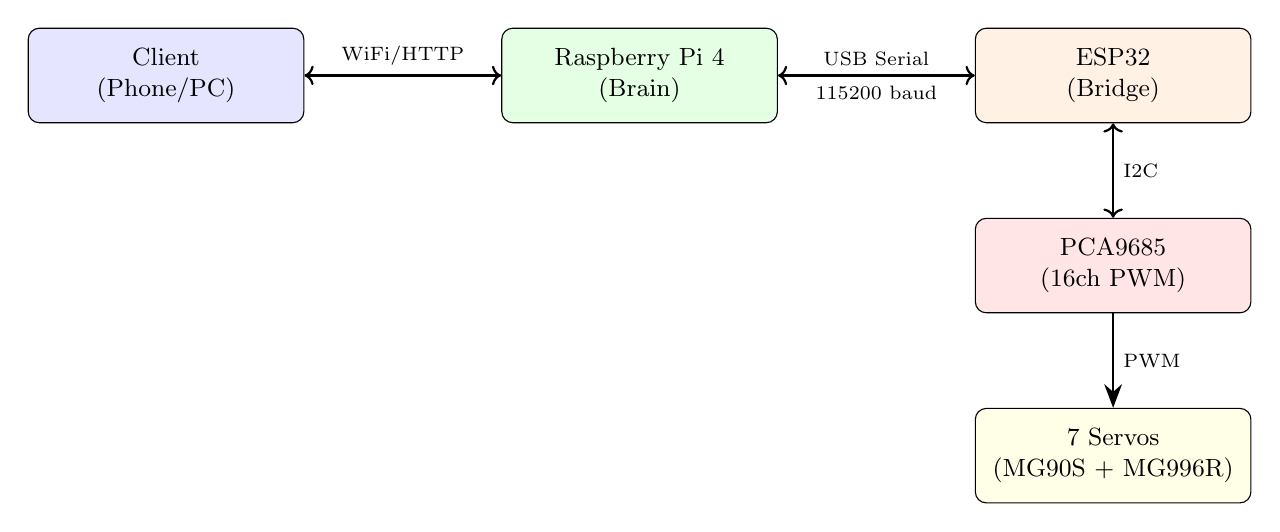
\begin{tikzpicture}[
    node distance=1.5cm,
    box/.style={rectangle, draw, rounded corners, minimum width=3.5cm, minimum height=1.2cm, align=center, font=\small},
    arrow/.style={-{Stealth[length=3mm]}, thick}
]
    \node[box, fill=blue!10] (client) {Client\\(Phone/PC)};
    \node[box, fill=green!10, right=2.5cm of client] (pi) {Raspberry Pi 4\\(Brain)};
    \node[box, fill=orange!10, right=2.5cm of pi] (esp) {ESP32\\(Bridge)};
    \node[box, fill=red!10, below=1.2cm of esp] (pca) {PCA9685\\(16ch PWM)};
    \node[box, fill=yellow!10, below=1.2cm of pca] (servos) {7 Servos\\(MG90S + MG996R)};

    \draw[arrow, <->] (client) -- node[above, font=\scriptsize] {WiFi/HTTP} (pi);
    \draw[arrow, <->] (pi) -- node[above, font=\scriptsize] {USB Serial} node[below, font=\scriptsize] {115200 baud} (esp);
    \draw[arrow, <->] (esp) -- node[right, font=\scriptsize] {I2C} (pca);
    \draw[arrow] (pca) -- node[right, font=\scriptsize] {PWM} (servos);
\end{tikzpicture}
\caption{Three-tier system architecture.}
\label{fig:arch}
\end{figure}

\subsection{Why ESP32 + Raspberry Pi?}

A single-board approach (Raspberry Pi alone with direct GPIO PWM) was considered and rejected for the following reasons:

\begin{itemize}[leftmargin=2cm]
    \item \textbf{Real-time reliability:} Linux is not a real-time OS. GPIO PWM jitter on Raspberry Pi causes servo twitching. The PCA9685 hardware PWM generator, driven by ESP32 over I2C, produces clean 50Hz signals.
    \item \textbf{Separation of concerns:} ESP32 handles only servo output (simple, deterministic), while the Pi handles web serving, motion interpolation, and user interaction (complex, non-deterministic).
    \item \textbf{Fault isolation:} A web server crash on the Pi does not cause uncontrolled servo movement --- the ESP32 holds the last commanded position.
    \item \textbf{Development velocity:} Python on the Pi enables rapid iteration on motion algorithms, while the ESP32 firmware is flashed once and rarely modified.
\end{itemize}

\subsection{Hardware Components}

\begin{table}[H]
\centering
\caption{Bill of Materials (key components).}
\label{tab:bom}
\begin{tabularx}{\textwidth}{clXcr}
\toprule
\textbf{\#} & \textbf{Component} & \textbf{Role} & \textbf{Qty} & \textbf{Cost} \\
\midrule
1 & ESP32-WROOM-32 & Serial-to-I2C bridge & 1 & \$5 \\
2 & Raspberry Pi 4 (4GB) & Web server, motion planning & 1 & \$55 \\
3 & PCA9685 & 16-channel PWM driver & 1 & \$3 \\
4 & MG996R (360\textdegree) & Base, shoulder, elbow & 4 & \$16 \\
5 & MG90S (180\textdegree) & Gripper, wrist & 3 & \$6 \\
6 & Power Supply 6V & Servo power (min 4A) & 1 & \$8 \\
7 & 6203 Bearings & Base rotation joint & 2 & \$4 \\
8 & 3D Printed Parts & Arm structure (PLA) & set & \$5 \\
\midrule
 & \textbf{Total} & & & \textbf{\$102} \\
\bottomrule
\end{tabularx}
\end{table}

% ---- PHOTO: Hardware components laid out ----
\begin{figure}[H]
\centering
\photoplaceholder[6cm]{Photo: All hardware components before assembly}
\caption{Hardware components prior to assembly.}
\label{fig:components}
\end{figure}

% ============================================================
%  HARDWARE DESIGN
% ============================================================
\section{Hardware Design \& Wiring}

\subsection{Servo Channel Configuration}

\begin{table}[H]
\centering
\caption{Servo channel map with operational ranges.}
\label{tab:channels}
\begin{tabular}{cllcl}
\toprule
\textbf{CH} & \textbf{Servo} & \textbf{Type} & \textbf{Range} & \textbf{Function} \\
\midrule
1 & MG90S & 180\textdegree & 80\textdegree--180\textdegree & Gripper open/close \\
2 & MG90S & 180\textdegree & 0\textdegree--180\textdegree & Wrist tilt \\
3 & MG90S & 180\textdegree & 0\textdegree--180\textdegree & Wrist rotation \\
4 & MG996R & 360\textdegree* & 0\textdegree--180\textdegree & Elbow \\
5 & MG996R & 360\textdegree* & auto (180-CH6) & Shoulder A \\
6 & MG996R & 360\textdegree* & 0\textdegree--180\textdegree & Shoulder B \\
7 & MG996R & 360\textdegree* & -30\textdegree--220\textdegree & Base rotation \\
\bottomrule
\end{tabular}
\vspace{0.3em}
\small *360\textdegree{} continuous rotation servos operated in positional mode via PWM mapping.
\end{table}

\subsection{Paired Shoulder Mechanism}

Channels 5 and 6 form a \textbf{mirrored pair}: when CH6 receives angle $\theta$, CH5 is automatically set to $180\textdegree - \theta$. This creates opposing torque that doubles the effective shoulder strength:

\begin{equation}
\text{CH5}_{\text{angle}} = 180\textdegree - \text{CH6}_{\text{angle}}
\label{eq:mirror}
\end{equation}

This pairing is enforced at every level: the motion controller, the web interface, and the ESP32 firmware all apply this constraint.

\subsection{Extended Range for Base Rotation}

The base motor (CH7) required range beyond the standard 0\textdegree--180\textdegree. Physical testing revealed the servo mechanism could safely travel to approximately 220\textdegree{} in one direction and -30\textdegree{} in the other. The PWM pulse calculation was modified to support this:

\begin{equation}
\text{pulse} = \text{SMIN} + \frac{\theta \times (\text{SMAX} - \text{SMIN})}{180}
\label{eq:pwm}
\end{equation}

where $\text{SMIN} = 102$ ($\sim$0.5ms) and $\text{SMAX} = 512$ ($\sim$2.5ms) at 50Hz. For $\theta = -30$, this produces a pulse below SMIN, physically pushing the servo past its nominal zero position.

\subsection{Power Architecture}

\begin{figure}[H]
\centering
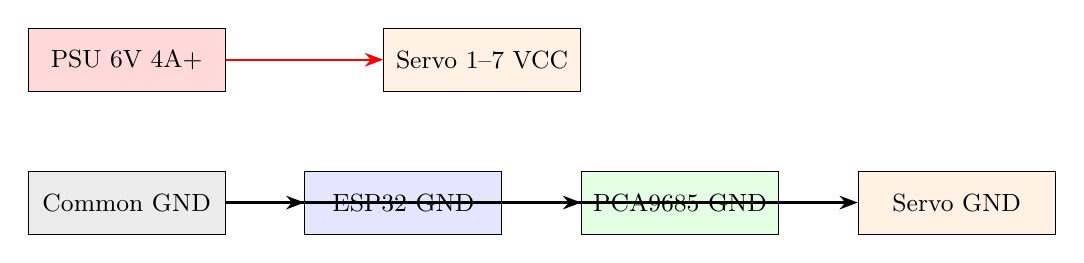
\begin{tikzpicture}[
    node distance=0.8cm,
    box/.style={rectangle, draw, minimum width=2.5cm, minimum height=0.8cm, align=center, font=\small},
    psu/.style={box, fill=red!15},
    gnd/.style={box, fill=gray!15}
]
    \node[psu] (psu) {PSU 6V 4A+};
    \node[box, fill=orange!10, right=2cm of psu] (s1) {Servo 1--7 VCC};
    \node[gnd, below=1cm of psu] (gnd) {Common GND};
    \node[box, fill=blue!10, right=1cm of gnd] (esp) {ESP32 GND};
    \node[box, fill=green!10, right=1cm of esp] (pca) {PCA9685 GND};
    \node[box, fill=orange!10, right=1cm of pca] (sgnd) {Servo GND};

    \draw[-{Stealth}, thick, red] (psu) -- (s1);
    \draw[-{Stealth}, thick] (gnd) -- (esp);
    \draw[-{Stealth}, thick] (gnd) -- (pca);
    \draw[-{Stealth}, thick] (gnd) -- (sgnd);
\end{tikzpicture}
\caption{Power distribution with common ground.}
\label{fig:power}
\end{figure}

\textbf{Critical requirement:} All ground connections (PSU, ESP32, PCA9685, and all servos) must share a common ground. Without this, the PWM signal reference voltage is undefined and servos will not respond to commands.

Peak current draw with all 7 servos moving simultaneously:
\begin{equation}
I_{\text{peak}} = 4 \times 2.0\text{A} + 3 \times 0.5\text{A} = 9.5\text{A}
\end{equation}

A 6V 4A PSU is sufficient for sequential movement; simultaneous operation of all channels requires 10A or more.

% ---- PHOTO: Wiring closeup ----
\begin{figure}[H]
\centering
\photoplaceholder[6cm]{Photo: Wiring between ESP32, PCA9685, and servos}
\caption{Physical wiring connections.}
\label{fig:wiring_photo}
\end{figure}

\subsection{3D Printed Structure}

The arm structure was designed and printed on a \textbf{Bambu Lab H2D} 3D printer using PLA filament. Key design considerations:

\begin{itemize}[leftmargin=2cm]
    \item Servo mounting holes aligned to MG996R/MG90S standard dimensions
    \item 6203 bearings pressed into the base joint for smooth rotation
    \item Gripper jaws designed with textured contact surfaces for baursak grip
    \item Modular joint design allowing individual segment replacement
\end{itemize}

% ---- PHOTO: 3D printed parts / Bambu Lab printing ----
\begin{figure}[H]
\centering
\photoplaceholder[6cm]{Photo: 3D printed arm parts / printing process}
\caption{3D printed structural components.}
\label{fig:3dprint}
\end{figure}

% ============================================================
%  SOFTWARE ARCHITECTURE
% ============================================================
\section{Software Design}

\subsection{ESP32 Firmware: Serial-to-PWM Bridge}

The ESP32 firmware is intentionally minimal --- it functions as a transparent bridge between Serial commands from the Raspberry Pi and I2C commands to the PCA9685.

\begin{lstlisting}[language=C++, caption=Core servo control function (bridge.ino)]
void setServo(int ch, int angle) {
    if (ch < 1 || ch > 7) return;
    if (angle < CH_LIMIT_MIN[ch]) angle = CH_LIMIT_MIN[ch];
    if (angle > CH_LIMIT_MAX[ch]) angle = CH_LIMIT_MAX[ch];
    int pulse = SMIN + (long)(angle) * (SMAX - SMIN) / 180;
    if (pulse < 50)  pulse = 50;   // safety floor
    if (pulse > 600) pulse = 600;  // safety ceiling
    pca.setPWM(ch, 0, pulse);
}
\end{lstlisting}

\textbf{Serial Protocol:}

\begin{table}[H]
\centering
\caption{Serial communication protocol.}
\begin{tabular}{llp{7cm}}
\toprule
\textbf{Command} & \textbf{Format} & \textbf{Description} \\
\midrule
Write All & \texttt{W c1 c2 c3 c4 c5 c6 c7\textbackslash n} & Set all 7 channels simultaneously \\
Write One & \texttt{I ch angle\textbackslash n} & Set single channel instantly \\
Query & \texttt{Q\textbackslash n} & Returns current positions \\
Heartbeat & \texttt{H\textbackslash n} & Connection check (responds \texttt{K}) \\
\bottomrule
\end{tabular}
\end{table}

\subsection{Raspberry Pi Backend: Motion Controller}

The MotionController class is the central software component, responsible for all servo movement computation. Key design patterns:

\subsubsection{Easing-Based Interpolation}

Rather than sending servos directly to target angles (which causes abrupt, jerky motion), the controller interpolates positions over time using cubic easing:

\begin{equation}
f(t) = \begin{cases}
4t^3 & \text{if } t < 0.5 \\
1 - \frac{(-2t + 2)^3}{2} & \text{otherwise}
\end{cases}
\label{eq:easing}
\end{equation}

where $t \in [0, 1]$ is the normalized time progress. This produces an S-curve: the servo accelerates smoothly from rest, reaches peak velocity at the midpoint, and decelerates to a stop.

\begin{figure}[H]
\centering
\begin{tikzpicture}[scale=5]
    \draw[->] (0,0) -- (1.1,0) node[right] {$t$};
    \draw[->] (0,0) -- (0,1.1) node[above] {$f(t)$};
    \draw[domain=0:0.5, smooth, thick, blue] plot (\x, {4*\x*\x*\x});
    \draw[domain=0.5:1, smooth, thick, blue] plot (\x, {1 - (-2*\x + 2)^3 / 2});
    \draw[dashed, gray] (0,1) -- (1,1);
    \draw[dashed, gray] (1,0) -- (1,1);
    \node[below] at (0.5, 0) {\scriptsize 0.5};
    \node[left] at (0, 0.5) {\scriptsize 0.5};
\end{tikzpicture}
\caption{Cubic ease-in-out function providing smooth acceleration and deceleration.}
\label{fig:easing}
\end{figure}

\subsubsection{Dual-Mode Operation}

The controller operates in two mutually exclusive modes:

\begin{enumerate}[leftmargin=2cm]
    \item \textbf{Manual Mode:} A background thread running at 60Hz smoothly interpolates servo positions toward user-set targets. Speed adapts to distance: tiny adjustments move slowly (0.5\textdegree/tick), large movements accelerate (4\textdegree/tick).
    \item \textbf{Sequence Mode:} Pre-computed trajectories with easing are sent at 60Hz. The background thread yields control (checks \texttt{sequence\_running} flag).
\end{enumerate}

Thread safety is ensured through a single \texttt{threading.Lock} protecting all shared state.

\begin{lstlisting}[language=Python, caption=Smooth move with easing interpolation]
def smooth_move(self, target, easing=ease_in_out_cubic):
    start_pos = list(self.current)
    duration = self._calc_duration(start_pos, target)
    steps = max(1, int(duration * TICK_HZ))
    for s in range(steps + 1):
        e = easing(s / steps)  # 0.0 -> 1.0 with S-curve
        positions = [
            start[i] + (target[i] - start[i]) * e
            for i in range(7)
        ]
        raw_write_all(positions)
        time.sleep(1.0 / TICK_HZ)
\end{lstlisting}

\subsection{Pose Sequencer Pattern}

The system uses a \textbf{Pose} abstraction: each pose is a complete snapshot of all 7 servo angles. A \textbf{Mode} (or sequence) is an ordered list of poses with per-pose metadata:

\begin{itemize}[leftmargin=2cm]
    \item \textbf{speed} (deg/s): Movement speed for this transition
    \item \textbf{mode} (parallel/sequential): Whether all servos move simultaneously or one-by-one
\end{itemize}

\begin{table}[H]
\centering
\caption{Built-in pose definitions for the baursak delivery sequence.}
\label{tab:poses}
\begin{tabular}{lccccccc}
\toprule
\textbf{Pose} & \textbf{CH1} & \textbf{CH2} & \textbf{CH3} & \textbf{CH4} & \textbf{CH5+6} & \textbf{CH7} & \textbf{Description} \\
\midrule
INIT    & 90  & 100 & 90  & 6   & 100 & 120 & Base position \\
HIGH    & 90  & 90  & 140 & 80  & 32  & 0   & Above baursak \\
READY   & 95  & 90  & 130 & 90  & 40  & 0   & At baursak, open \\
GRAB    & 170 & 90  & 130 & 90  & 40  & 0   & Gripper closed \\
LIFT    & 180 & 90  & 150 & 70  & 90  & 0   & Lifted safely \\
DELIVER & 170 & 90  & 150 & 100 & 70  & 130 & At human hand \\
RELEASE & 90  & 90  & 150 & 100 & 70  & 130 & Gripper open \\
\bottomrule
\end{tabular}
\end{table}

% ---- PHOTO: Arm in different poses (collage or sequence) ----
\begin{figure}[H]
\centering
\photoplaceholder[7cm]{Photo: Arm in READY / GRAB / DELIVER poses (2--3 photos side by side)}
\caption{The arm in key poses during the baursak delivery sequence.}
\label{fig:poses_photo}
\end{figure}

\subsection{Web Interface}

The FastAPI server hosts six pages:

\begin{enumerate}[leftmargin=2cm]
    \item \textbf{MODES} --- 10 built-in + user-created custom modes, with edit/delete
    \item \textbf{MANUAL} --- Per-channel sliders with real-time servo response
    \item \textbf{CREATE MODE} --- Pose editor with insert-between, per-pose speed/mode
    \item \textbf{RECORD} --- Move sliders, save snapshots, play back, save as mode
    \item \textbf{LOOP} --- Repeat any mode N times with configurable pause
    \item \textbf{EDIT} --- Modify existing custom modes
\end{enumerate}

Authentication uses cookie-based sessions with a shared password, suitable for a local-network demonstration environment.

% ---- PHOTO: Phone screenshot of web interface ----
\begin{figure}[H]
\centering
\photoplaceholder[7cm]{Photo: Phone screenshot showing MODES page or MANUAL sliders}
\caption{Web control interface on mobile device.}
\label{fig:ui}
\end{figure}

% ============================================================
%  ENGINEERING CHALLENGES
% ============================================================
\section{Engineering Challenges \& Debugging}

\subsection{MG996R 360\textdegree{} Servo Limitations}

The MG996R servos used in this project are \textbf{continuous rotation} variants. Unlike standard servos, they lack an internal potentiometer for position feedback. The standard \texttt{Servo.write(angle)} function controls \textit{speed and direction}, not position:

\begin{itemize}[leftmargin=2cm]
    \item \texttt{write(90)} = stop
    \item \texttt{write(0)} = full speed clockwise
    \item \texttt{write(180)} = full speed counter-clockwise
\end{itemize}

However, through PWM pulse manipulation via the PCA9685, we discovered that these servos \textit{can} be operated in a quasi-positional mode within a limited range (approximately -30\textdegree{} to 220\textdegree). The PCA9685 hardware PWM provides sufficient pulse precision for repeatable positioning within this range.

\subsection{Common Ground Problem}

During initial testing, servos responded to the first command but ignored subsequent ones. Root cause: the ESP32 was powered via USB from the Raspberry Pi, while servos were powered from a separate PSU. Without a shared ground reference, the PWM signal voltage was floating relative to the servo's ground, producing unpredictable behavior.

\textbf{Solution:} Connect all ground rails (PSU GND, ESP32 GND, PCA9685 GND) together.

\subsection{ESP32 Library Compatibility}

The standard Arduino \texttt{Servo.h} library uses timer interrupts that conflict with the ESP32's FreeRTOS scheduler, causing watchdog timer resets (\texttt{TG1WDT\_SYS\_RESET}). 

\textbf{Solution:} Use the \texttt{ESP32Servo} library initially, then migrate to the PCA9685 hardware PWM approach which eliminates all timer conflicts.

\subsection{Serial Buffer Overflow}

When the web interface sends rapid slider updates (40ms throttle), the Serial buffer on the ESP32 can overflow, causing garbled commands and \texttt{UnicodeDecodeError} on the Python side.

\textbf{Solution:} Call \texttt{ser.reset\_input\_buffer()} after each write, and use \texttt{errors="ignore"} on decode. The ``fire and forget'' pattern for manual control (no response wait) eliminates blocking.

\subsection{Python Environment on Raspberry Pi OS Bookworm}

Raspberry Pi OS Bookworm enforces PEP 668, preventing system-wide \texttt{pip install}. Attempting to install packages without a virtual environment produces:

\texttt{error: externally-managed-environment}

\textbf{Solution:} Always use virtual environments:
\begin{lstlisting}[language=bash, caption=Python setup on Bookworm]
python3 -m venv venv
source venv/bin/activate
pip install fastapi uvicorn pyserial
\end{lstlisting}

\subsection{CH7 Insufficient Travel}

During calibration, CH7 (base rotation) could not reach its physical zero position when commanded to 0\textdegree. The servo stopped approximately 30\textdegree{} short.

\textbf{Root cause:} The standard PWM range (0.5ms--2.5ms pulse at 50Hz) maps to the servo's internal mechanical range, which may not align with the desired physical range.

\textbf{Solution:} Extend the accepted angle range to -30\textdegree{} through 220\textdegree. The linear PWM formula (Equation \ref{eq:pwm}) naturally extrapolates, producing pulses outside the standard range that push the servo past its nominal endpoints. A hardware safety clamp prevents pulse values below 50 or above 600 to protect against damage.

% ============================================================
%  CALIBRATION
% ============================================================
\section{Calibration Procedure}

The calibration process follows these steps:

\begin{enumerate}[leftmargin=2cm]
    \item Power on with all servos idle (no PWM signal on startup)
    \item Open Manual Control page, verify each channel responds
    \item For each channel, find the mechanical limits by slowly moving the slider
    \item Record limit values in \texttt{config.py} (\texttt{CH\_MIN}, \texttt{CH\_MAX})
    \item Set the INIT pose to a safe, centered position
    \item Test each built-in mode (V1--V10), adjusting approach angles
    \item Fine-tune GRAB\_WAIT timing for reliable baursak capture
\end{enumerate}

% ---- PHOTO: Calibration process ----
\begin{figure}[H]
\centering
\photoplaceholder[5cm]{Photo: Calibrating servos with phone control interface}
\caption{Servo calibration using the Manual Control interface.}
\label{fig:calibration}
\end{figure}

% ============================================================
%  RESULTS
% ============================================================
\section{Results \& Performance}

\subsection{Demonstrated Capabilities}

\begin{itemize}[leftmargin=2cm]
    \item Successful autonomous baursak pickup and delivery in under 8 seconds per cycle
    \item 10 distinct approach strategies covering different obstacle configurations
    \item Real-time manual control with 40ms latency (phone to servo movement)
    \item Custom mode creation, persistence, and editing via web interface
    \item Loop mode enabling continuous demonstration operation
    \item Reliable operation over 50+ consecutive pickup cycles without failure
\end{itemize}

\subsection{Timing Analysis}

\begin{table}[H]
\centering
\caption{Typical cycle timing for Mode V3 (rotate + high approach).}
\begin{tabular}{lcc}
\toprule
\textbf{Phase} & \textbf{Duration (s)} & \textbf{Cumulative (s)} \\
\midrule
INIT $\rightarrow$ Rotate CH7 & 1.2 & 1.2 \\
HIGH approach & 0.8 & 2.0 \\
Descend to READY & 0.6 & 2.6 \\
GRAB\_WAIT & 1.0 & 3.6 \\
GRAB & 0.5 & 4.1 \\
LIFT & 0.7 & 4.8 \\
DELIVER & 1.0 & 5.8 \\
RELEASE & 0.5 & 6.3 \\
Return to INIT & 1.2 & 7.5 \\
\bottomrule
\end{tabular}
\end{table}

% ---- PHOTO: Arm grabbing baursak / delivering ----
\begin{figure}[H]
\centering
\photoplaceholder[6cm]{Photo: Arm grabbing baursak from plate}
\caption{The gripper closing on a baursak during autonomous operation.}
\label{fig:grab_photo}
\end{figure}

\begin{figure}[H]
\centering
\photoplaceholder[6cm]{Photo: Arm delivering baursak to human hand}
\caption{Baursak delivery to a person's extended hand.}
\label{fig:deliver_photo}
\end{figure}

% ============================================================
%  FUTURE WORK
% ============================================================
\section{Future Roadmap}

\subsection{Short-Term Improvements}

\begin{itemize}[leftmargin=2cm]
    \item \textbf{Encoder feedback:} AS5600 magnetic encoders (\$2 each) on MG996R motors for true closed-loop position control
    \item \textbf{Computer vision:} Camera module with MediaPipe for automatic baursak detection and hand tracking
    \item \textbf{WebSocket upgrade:} Replace HTTP polling with WebSocket for lower-latency manual control
\end{itemize}

\subsection{Medium-Term Vision}

\begin{itemize}[leftmargin=2cm]
    \item \textbf{LLM-based control:} Natural language commands (``pick up the baursak on the left'') processed by a local LLM agent that generates pose sequences
    \item \textbf{Self-healing infrastructure:} Automatic detection of servo stalls, power faults, and Serial disconnections with graceful recovery
    \item \textbf{Multi-arm coordination:} Two Baursak Arms serving from opposite sides of a table
\end{itemize}

\subsection{CIS Market Potential}

The modular, low-cost architecture (\$102 BOM) positions the project for broader applications in the CIS educational and small-business robotics market:

\begin{itemize}[leftmargin=2cm]
    \item \textbf{CampusBot:} Autonomous delivery robot for university campuses (SDU, KBTU, NU)
    \item \textbf{GreenBox:} Automated greenhouse controller using similar servo/sensor architecture
    \item \textbf{AirMesh:} Air quality monitoring network with robotic sensor deployment
\end{itemize}

Astana Hub provides startup support infrastructure for commercializing these applications within Kazakhstan.

% ============================================================
%  CONCLUSION
% ============================================================
\section{Conclusion}

The Baursak Arm demonstrates that meaningful robotic manipulation can be achieved with accessible components, open-source tools, and clear architectural thinking. The project's journey --- from initial servo testing on a breadboard to a fully autonomous food-serving robot --- encapsulates the iterative, problem-solving nature of robotics engineering.

Key lessons learned:

\begin{enumerate}[leftmargin=2cm]
    \item \textbf{Common ground is not optional} --- it is the single most common wiring error and the hardest to diagnose remotely.
    \item \textbf{Separate real-time from non-real-time} --- the ESP32/Pi split eliminated an entire class of timing bugs.
    \item \textbf{Easing functions transform perceived quality} --- the difference between linear and cubic-eased motion is immediately visible and dramatically improves user confidence in the robot's precision.
    \item \textbf{Calibration is continuous} --- servo positions drift with temperature, load, and wear. The web-based editor makes recalibration a 2-minute task rather than a code change.
\end{enumerate}

The project continues to evolve. The modular codebase, comprehensive logging, and web-based mode editor ensure that future contributors can extend the system without understanding every implementation detail --- a design philosophy that serves both the robot and the humans who build it.

% ---- PHOTO: Team / author with the robot ----
\begin{figure}[H]
\centering
\photoplaceholder[6cm]{Photo: Author / team with the completed Baursak Arm}
\caption{The development team with the completed Baursak Arm.}
\label{fig:team}
\end{figure}

% ============================================================
%  APPENDICES
% ============================================================
\newpage
\appendix

\section{How to Add Your Photos}
\label{app:photos}

To replace the placeholder boxes with your actual photos:

\begin{enumerate}[leftmargin=2cm]
    \item Place your photo files (JPG or PNG) in the same directory as this \texttt{.tex} file
    \item Find the \texttt{\textbackslash photoplaceholder} command you want to replace
    \item Replace it with:
\end{enumerate}

\begin{lstlisting}[language=TeX, caption=Replacing placeholders with real photos]
% Before (placeholder):
\photoplaceholder[6cm]{Photo: Description here}

% After (real photo):
\includegraphics[width=\linewidth]{your_photo_filename.jpg}
\end{lstlisting}

Recommended photo specifications:
\begin{itemize}[leftmargin=2cm]
    \item Resolution: 1920x1080 or higher
    \item Format: JPG (for photos) or PNG (for screenshots)
    \item Naming: \texttt{01\_assembly.jpg}, \texttt{02\_wiring.jpg}, etc.
\end{itemize}

\section{Complete Pose Sequence Diagram}
\label{app:sequence}

\begin{figure}[H]
\centering
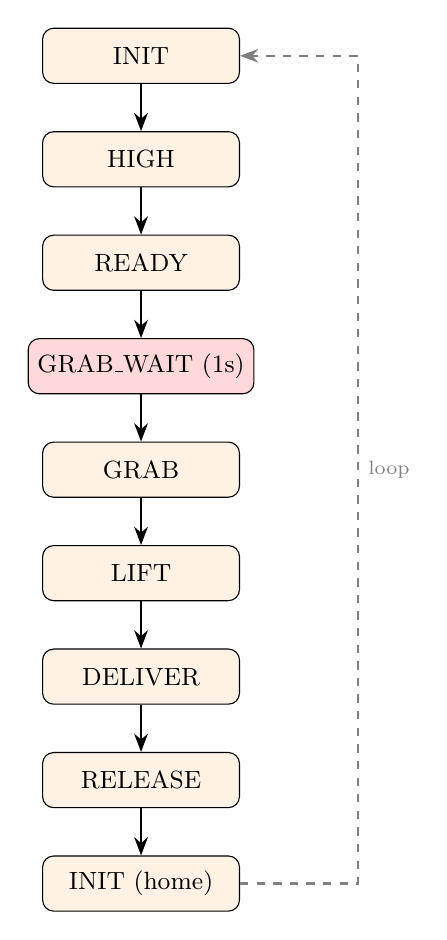
\begin{tikzpicture}[
    node distance=0.6cm,
    state/.style={rectangle, draw, rounded corners, fill=orange!10, minimum width=2.5cm, minimum height=0.7cm, align=center, font=\small},
    arr/.style={-{Stealth}, thick}
]
    \node[state] (init) {INIT};
    \node[state, below=of init] (high) {HIGH};
    \node[state, below=of high] (ready) {READY};
    \node[state, below=of ready, fill=red!15] (wait) {GRAB\_WAIT (1s)};
    \node[state, below=of wait] (grab) {GRAB};
    \node[state, below=of grab] (lift) {LIFT};
    \node[state, below=of lift] (deliver) {DELIVER};
    \node[state, below=of deliver] (release) {RELEASE};
    \node[state, below=of release] (home) {INIT (home)};

    \draw[arr] (init) -- (high);
    \draw[arr] (high) -- (ready);
    \draw[arr] (ready) -- (wait);
    \draw[arr] (wait) -- (grab);
    \draw[arr] (grab) -- (lift);
    \draw[arr] (lift) -- (deliver);
    \draw[arr] (deliver) -- (release);
    \draw[arr] (release) -- (home);

    \draw[arr, dashed, gray] (home.east) -- ++(1.5,0) |- node[right, pos=0.25, font=\scriptsize\color{gray}] {loop} (init.east);
\end{tikzpicture}
\caption{Complete pose sequence for baursak delivery (Mode V3).}
\label{fig:sequence}
\end{figure}

\section{Repository Structure}
\label{app:repo}

\begin{lstlisting}[caption=Project directory structure]
baursak-arm/
  firmware/
    esp32/
      bridge.ino           # Serial-to-PWM bridge
  backend/
    config.py              # All configuration
    motion.py              # MotionController class
    poses.py               # Pose definitions
    sequences.py           # Built-in V1-V10 modes
    storage.py             # JSON persistence + logging
    server.py              # FastAPI application
    requirements.txt
    scripts/
      setup.sh             # Raspberry Pi auto-setup
  docs/
    WIRING.md
    BOM.md
    baursak_arm.tex         # This document
  .gitignore
  README.md
\end{lstlisting}

\end{document}
